%!TEX root = Main.tex
\chapter{Implementation}
The following chapter seeks to explain the implementation of the mini project.\\

\section{Overall Design}
Image and explaination of the overall system and blocks\\

\section{Serial communication}
The serial communication is responsible for the transfer of the image to and from the Telos B. A header file is available to both the PC software and the Telos B program. It contains a series of defines that are used for the communication messages. The defines can be found in table \ref{definetable}.
\begin{table}[H]
    \begin{tabular}{|l|l|l|}
    \hline
    Name                  & Val & Description                                               \\ \hline
    TRANSFER\_TO\_TELOS   & 1     & Used to tell the Telos B to prepare to receive the image. \\ \hline
    TRANSFER\_OK          & 2     & Used to tell the PC that the transfer was ok.             \\ \hline
    TRANSFER\_FAIL        & 3     & Used to tell the PC that the transfer failed.             \\ \hline
    TRANSFER\_READY       & 4     & Used to tell the PC that the transfer can be initiated.   \\ \hline
    TRANSFER\_FROM\_TELOS & 5     & Used to tell the Telos B to transfer the image to the PC.  \\ \hline
    TRANSFER\_DONE        & 6     & Used to tell the PC that the image transfer is done.      \\ \hline
    \end{tabular}
    \caption{Defines for serial communication.}
    \label{definetable}
\end{table}
\begin{figure}[H]
	\centering
	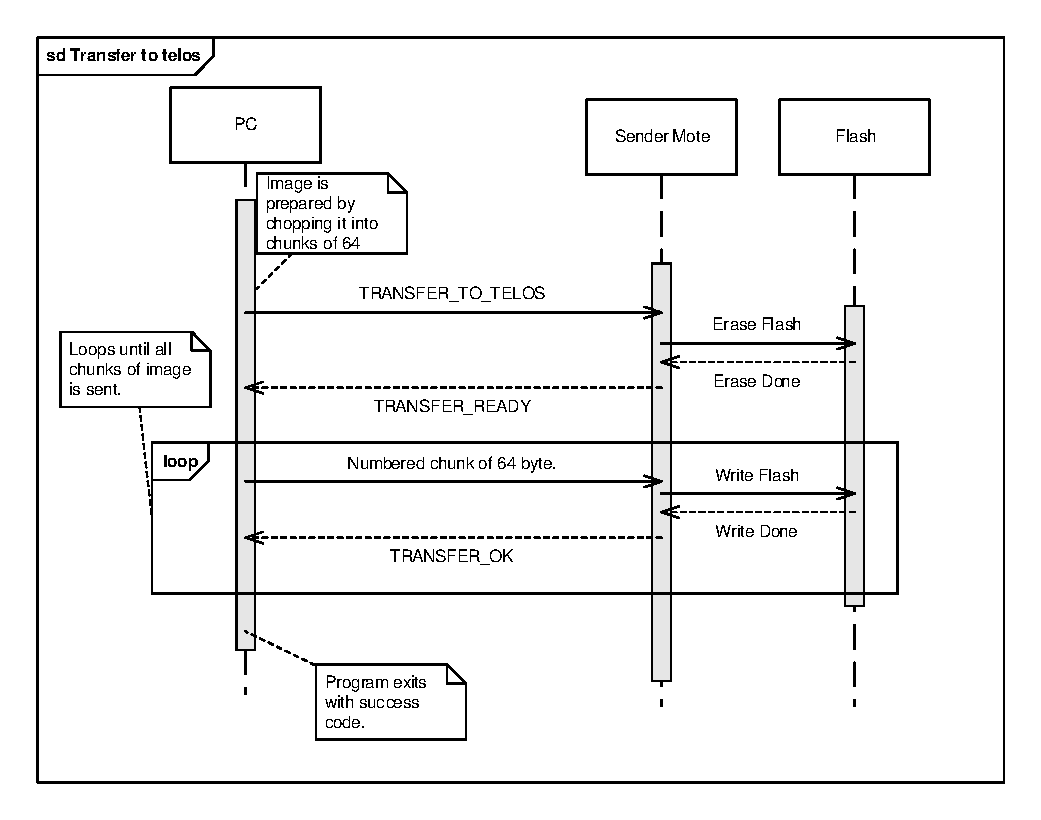
\includegraphics[width=0.8\textwidth]{PCtoTelosb}
	\caption{Transfer to telos sequence diagramme.}
	\label{transfertotelos}
\end{figure}

\begin{figure}[H]
	\centering
	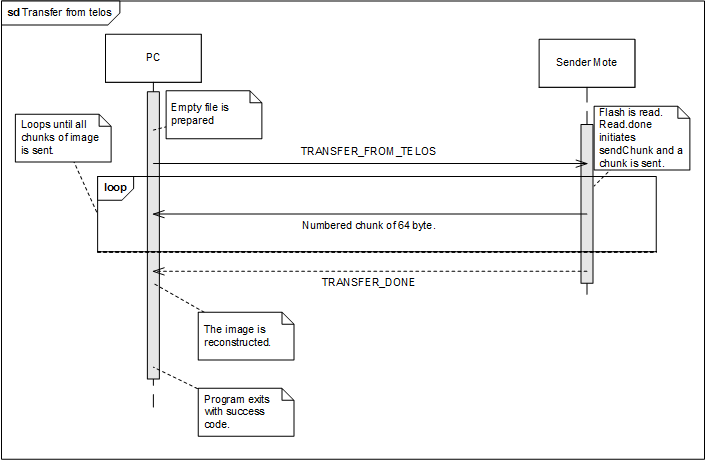
\includegraphics[width=0.8\textwidth]{PCfromTelosb}
	\caption{Transfer from telos sequence diagramme.}
	\label{transferfromtelos}
\end{figure}

\section{Radio Block}

\section{Compression block}


